\section{Theorie}

\begin{flushleft}
    Brückenschaltungen sind eine häufig verwendete Methode in der Messtechnik, weil diese die Auflösung einer Messung erhöhen.
    Durch Verwenden der Nullmethode gelingt dies insbesondere.
    In diesem Versuch wird die Nullmethode durch die abgeglichenen Brücken realisiert.
    Ebenso sind jegliche physikalische Größen gut messbar, wenn diese sich als elektrischer Widerstand, bzw. als Impedanz, darstellen lassen.  
\end{flushleft}

\begin{flushleft}
    Um die Brückenspannung und die dazugehörige Abgleichbedingung zu berechnen, untersucht man die Potentialdifferenz der Schaltung, welche in zwei Punkten auf zwei getrennten stromdurchflossenen Leitern gemessen wird. 
    Diese Potentialdifferenz steht in Abhängigkeit mit dem Widerstandsverhältnis der Schaltung. 
    Eine „normale“ Brückengleichung ist in Abbildung \ref{Abbildung1} zu sehen.
\end{flushleft}

\begin{figure}[H]
    \centering
    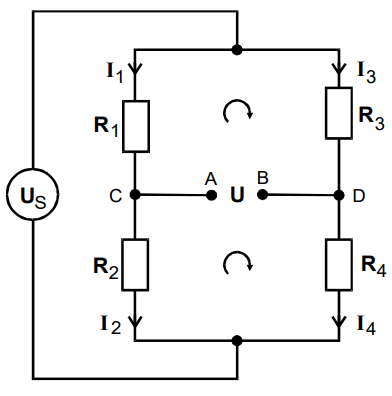
\includegraphics[height=80mm]{bilder/Abbildung1.png}
    \caption{Eine Abbildung einer einfachen Brückenschaltung \cite{a1}. \label{Abbildung1} }
\end{figure}

\begin{flushleft}
    Die Spannung $U$ zwischen den beiden Punkten wird als Brückenspannung bezeichnet. 
    Die Berechnung dieser Spannung beruht auf den zwei Kirchhoffschen Gesetzen. \\
    Das erste Kirchhoffsche Gesetz besagt, dass die Summe der zufließenden Ströme gleich der Summe der abfließenden Ströme in einem Verzweigungspunkt ist.
\end{flushleft}

\begin{align*}
    \sum \limits_{\text{k}} I_{\text{k}} = 0 \\
\end{align*}

\begin{figure}[H]
    \centering
    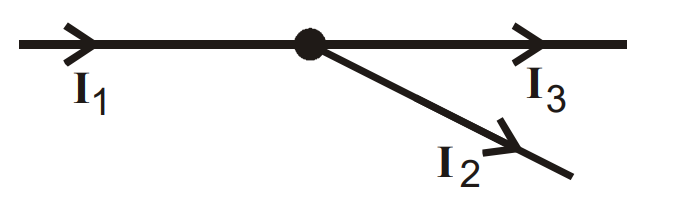
\includegraphics[height=15mm]{bilder/Abbildung2.png}
    \caption{Die Abbildung eines Knotenpunktes mit einer Leiterverzeigung \cite{a1}.\label{Abbildung2} }
\end{figure}

\begin{flushleft}
    Das zweite Kirchhoffsche Gesetz besagt, dass die Summe aller Spannungen einer beliebig gewählten Masche des Schaltkreises gleich null ist. 
\end{flushleft}

\begin{align*}
    \sum \limits_{\text{k}} U_{\text{k}} = 0. 
\end{align*}

\begin{figure}[H]
    \centering
    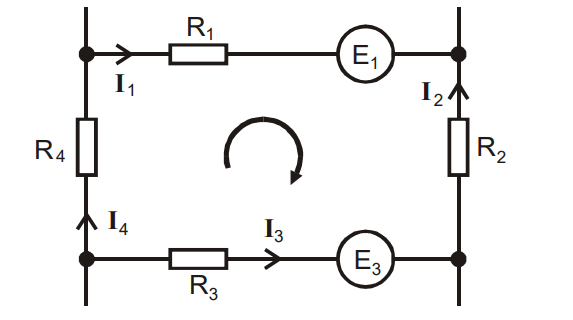
\includegraphics[height=40mm]{bilder/Abbildung3.png}
    \caption{Die Abbildung einer Masche \cite{a1}.\label{Abbildung3} }
\end{figure}

\begin{flushleft}
    Wenn der Strompfeil im Uhrzeigersinn läuft, ist die Spannung positiv zu rechnen. Wenn der Strompfeil gegen den Uhrzeigersinn läuft, ist die Spannung negativ zu rechnen.
\end{flushleft}

\begin{align}
    \intertext{Durch die beiden Kirchhoffschen Gesetze ergibt sich die Formel für die Brückenspannung in Abhängigkeit von den
    Schaltungsparametern}
    U_{\text{Br}} = \frac{R_{2}R_{3} - R_{1}R_{4}}{(R_{3} + R_{4})(R_{1} + R_{2})}U_{\text{S}}
    \intertext{mit}
    U_{\text{s}} = I_{1}(R_{1} + R_{2}).
\end{align}

\begin{flushleft}  
    Wenn die Widerstände so gewählt werden, dass die Brückenspannung, welche unabhängig von der Speisespannung ist, verschwindet,
    ergibt sich die sogenannte Abgleichbedingung:
\end{flushleft}

\begin{align*}
    R_{1}R_{4} = R_{2}R_{3}.
\end{align*}

\begin{align*}
    \intertext{Ebenfalls wichtig sind die Impedanzen bei Brückenschaltungen.
    Unter einer Impedanz wird die Zusammenarbeit von Blind- und Wirkwiderstand verstanden.
    Der Wirkwiderstand X steht hierbei für den Realteil und der Blindwiderstand Y für den imaginären Teil.}
    \xi = \text{X} + \text{iY}
\end{align*}

\subsection{Wheatstonesche Brücke}

\begin{flushleft}
    Die Wheatstonesche Brücke ist eine Widerstandsmessbrücke und enthält dadurch nur ohmsche Widerstände.
    Betrieben kann diese mit Gleich- sowie Wechselstrom, wobei der Nullindikator entsprechend der Stromart gewählt werden muss. 
    In Abbildung \ref{4} ist die Wheatstonesche Brückenschaltung gezeigt. 
\end{flushleft}

\begin{figure}[H]
    \centering
    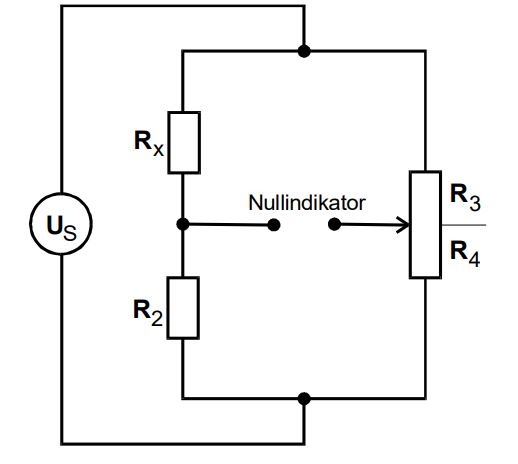
\includegraphics[height=60mm]{bilder/Abbildung4.png}
    \caption{Die Abbildung einer Wheatstonesche Brücke \cite{a1}. \label{Abbildung4}}
\end{figure}

\begin{align}
    \intertext{Die Bestimmung des unbekannten Widerstandes erfolgt durch die Formel}
    R_{x} = R_{2} \cdot  \frac{R_{3}}{R_{4}}.  \label{3}
\end{align}


\subsection{Kapazitätsmessbrücke}

\begin{flushleft}
    Die Kapazitätsmessbrücke ist eine Schaltung, in welcher Kondensatoren hinzugefügt werden. 
    Durch den Kondensator, welcher neben dem Speichern von Energie auch andere Eigenschaften mit sich bringt, wie die Umwandlung von elektrischer Energie zu Wärmeenergie.
    Der Kondensator ist in Reihe mit einem ohmschen Widerstand geschaltet, aufgrund der Eigenschaft des realen Kondensators.
    Das Schaltkreisbild der Kapazitätmessbrücke ist  zu sehen in Abbildung \ref{Abbildung5}. 
\end{flushleft}

\begin{figure}[H]
    \centering
    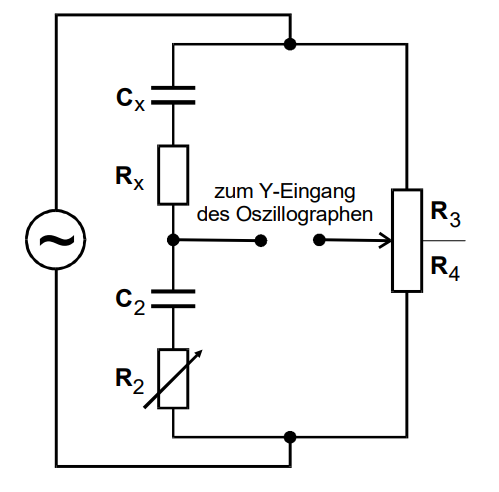
\includegraphics[height=60mm]{bilder/Abbildung5.png}
    \caption{Die Abbildung einer Kapazitätsmessbrücke \cite{a1}. \label{Abbildung5} }
\end{figure}

\begin{align}
    \intertext{Die Abgleichbedingung für die Kapazitätmessbrücke lauten}
    R_{x} = R_{2}\frac{R_{3}}{R_{4}}  \label{4}
    \intertext{und}
    C_{x} = C_{2}\frac{R_{4}}{R_{3}}. \label{5}
\end{align}

\subsection{Induktivitätsmessbrücke}

\begin{flushleft}
    Bei der Induktivitätsbrücke wird in dem Schaltbild der Kapazitätmessbrücke der Kondensator durch eine Spule ersetzt, 
    welche ein Teil der magnetischen Feldenergie in Wärme umwandelt. 
\end{flushleft}


\begin{figure}[H]
    \centering
    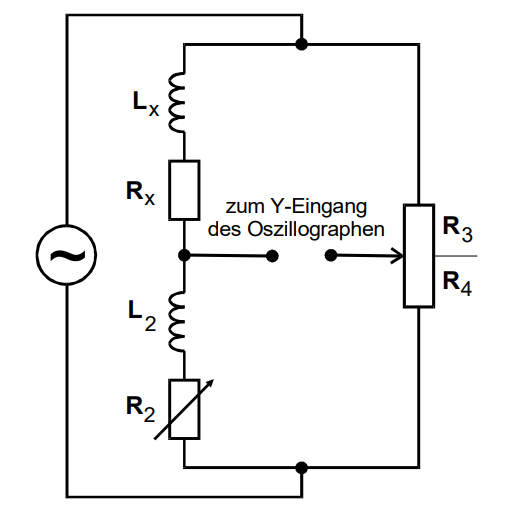
\includegraphics[height=60mm]{bilder/Abbildung6.png}
    \caption{Die Abbildung einer Induktivitätsmessbrücke    \cite{a1}. \label{Abbildung6} }
\end{figure}

\begin{align}
    \intertext{Die Abgleichbedingung für $R_{x}$ ist identisch mit der, der Kapazitätsmessbrücke, für die Induktivität gilt jedoch}
    L_{x} = L_{2}\frac{R_{3}}{R_{4}}. \label{6}
\end{align}

\subsection{Maxwell-Brücke}

\begin{flushleft}
    Die Maxwell-Brücke ist eine weitere Induktivitätsmessbrücke, welche für die Messung der Induktivität verwendet wird.
    Hierbei fällt die Spule $L_{2}$ weg, weil die Spule möglichst geringe Verluste vorweisen sollte und dadurch der Widerstand $R_{2}$ den Wirkanteil realisiert.
    Bei niedrigen Frequenzen ist dies jedoch schwer zu realisieren, weswegen man die Maxwell-Brücke verwendet. 
    Der Widerstand $R_{2}$ wird als bekannten Widerstand genommen, aufgrund der möglichst verlustarmen Kapazität $C_{4}$,
    $R_{3}$ und $R_{4}$ sind beide Regelwiderstände, wobei $R_{4}$ parralell zu dem Kondensator $C_{4}$ geschaltet ist. 
    Das Schaltbild zu der Maxwell-Brücke wird in Abbildung \ref{Abbildung7} gezeigt.
\end{flushleft}


\begin{figure}[H]
    \centering
    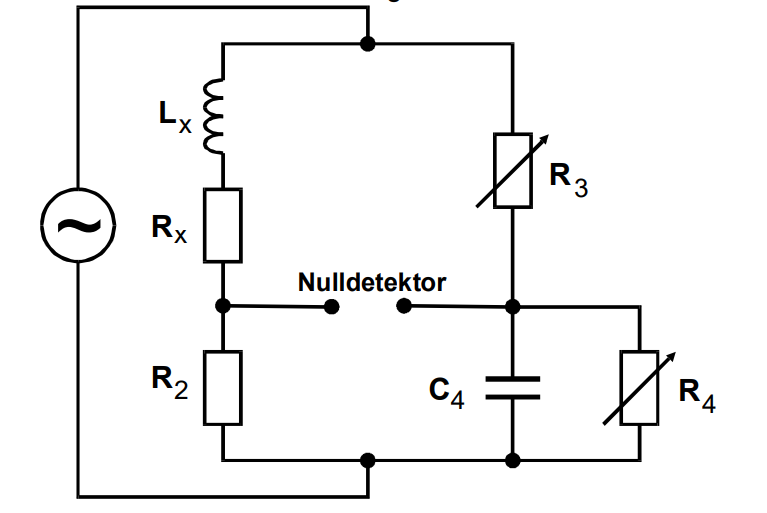
\includegraphics[height=60mm]{bilder/Abbildung7.png}
    \caption{Die Abbildung einer Maxwell-Brücke    \cite{a1}. \label{Abbildung7} }
\end{figure}

\begin{align}
    \intertext{Die Abgleichbedingungen für die Maxwell-Brücke ergeben sich durch}
    R_{x} = \frac{R_{2}R_{3}}{R_{4}} \label{7}
    \intertext{und}
    L_{x} = R_{2}R_{3}C_{4}. \label{8}
\end{align}

\subsection{Wien-Robinson-Brücke}


\begin{flushleft}
    Die Wien-Robinson-Brücke verfügt über keine Abgleichelemente, was bedeutet, dass alle Impedanzen bekannt sind.
    Deswegen sollten die Bauteile dieser Schaltung, $C$, $R$ und $R'$, eine möglichst geringe Toleranz haben.
    Die Kondensatoren sollten dazu ebenfalls geringe Verluste haben.
    Durch das Ändern der Frequenz wird bei dieser Schaltung dieser Abgleich durchgeführt, was bedeutet, dass die Wien-Robinson-Brücke als elektronischer Filter funktioniert.
    Deutlich wird dies in der Aufstellung der Gleichung für das Verhältnis der Brückenspannung zur Speisespannung.
\end{flushleft}


\begin{figure}[H]
    \centering
    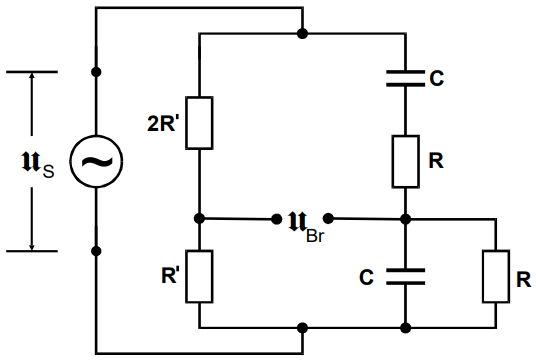
\includegraphics[height=60mm]{bilder/Abbildung8.png}
    \caption{Die Abbildung einer Wien-Robinson-Brücke \cite{a1}. \label{Abbildung8} }
\end{figure}

\begin{align*}
    \intertext{Die Brückenspannung setzt sich hierbei zusammen aus}
    U_{\text{Br}} = \frac{\omega^2 R^2 C^2 - 1 }{3\left(1 - \omega^2 R^2 C^2\right) + 9 i \omega R C}U_{\text{S}}. \label{9}
\end{align*}

\begin{align}
    \intertext{Das darausfolgende Verhältnis zwischen Speise- und Brückenspannung }
    \left\lvert \frac{U_{\text{Br}}}{U_{\text{Sp}}} \right\rvert^2 = \frac{\left(\omega^2 R^2 C^2 -1\right)}{9 \left(\left(1 - \omega^2 R^2 C^2\right)^2 + 9\omega^2 R^2 C^2\right)}
\end{align}

\begin{align*}
    \intertext{mit}
    \omega_{0} = \frac{1}{RC}
    \intertext{und dem Frequenzverhältnis}
    \unit{\ohm} = \omega \mathbin{/} \omega_{0}
\end{align*}

\begin{align}
    \intertext{wird die Gleichung (\ref{9}) vereinfacht zu}
    \left\lvert \frac{U_{\text{Br}}}{U_{\text{Sp}}} \right\rvert^2 = \frac{1}{9} \frac{\left(\unit{\ohm}^2 - 1\right)^2}{\left(1 - \unit{\ohm}^2 \right) + 9\,\unit{\ohm}^2 }. \label{10}
\end{align}

\begin{align*}
    \intertext{Bei einer Frequenz von $\omega_{0}$ sollte keine Brückenspannung mehr zu sehen sein.
    In der Theorie klappt es, aber in der Realität wird trotzdem ein minimaler Wert angegeben, der sich durch Oberwellen erklären lässt
    Das Verhältnis von Oberwellengehalt zur Grundwelle wird durch den Klirrfaktor ausgedrückt:}
\end{align*}

\begin{equation}
    \kappa = \frac{\sqrt{\sum \limits_{i=2}^N U_{i}^2 }}{U_{1}} \label{11}
\end{equation}